\documentclass[12pt]{article}

\usepackage{amsmath}    % need for subequations
\usepackage{mathtools}  % need for math tools
\usepackage{amsmath}    % need for subequations
\usepackage{graphicx}   % need for figures
\usepackage{verbatim}   % useful for program listings
\usepackage{color}      % use if color is used in text
\usepackage{hyperref}   % use for hypertext links, including those to external documents and URLs
\usepackage{natbib}     % Used for Bibliography
\usepackage{ifthen}

% Names
\def\XCat{{\sc XCat}}

% Physical constants.
\def\G{{\rm G}}
\def\clight{{\rm c}}
\def\d{{\rm d}}
\def\e{{\rm e}}

% AdS
\newcounter{AdSDone}
\setcounter{AdSDone}{0}
\def\AdS{\ifthenelse{\equal{\arabic{AdSDone}}{0}}{anti de Sitter (AdS)\setcounter{AdSDone}{1}}{AdS}}

\title{\XCat\ Report}
\author{\copyright 2013 by Arya Farahi\thanks{E-mail: {\tt aryaf@umich.edu}}}
\date{\today}

\begin{document}
\maketitle

\begin{abstract}
In progress ...
\end{abstract}


\section{Introduction}

\XCat\ is an open source code for data analysing of X-Ray observational data of variouse fields in AdS spaces. It is developed in 2013 by Arya Farahi for ... project under guidance of August E. Evrard at University of Michigan - Ann Arbor.  
\section{Results}
\subsection{Final Plots}

\begin{figure}[hbt]
 \centering
 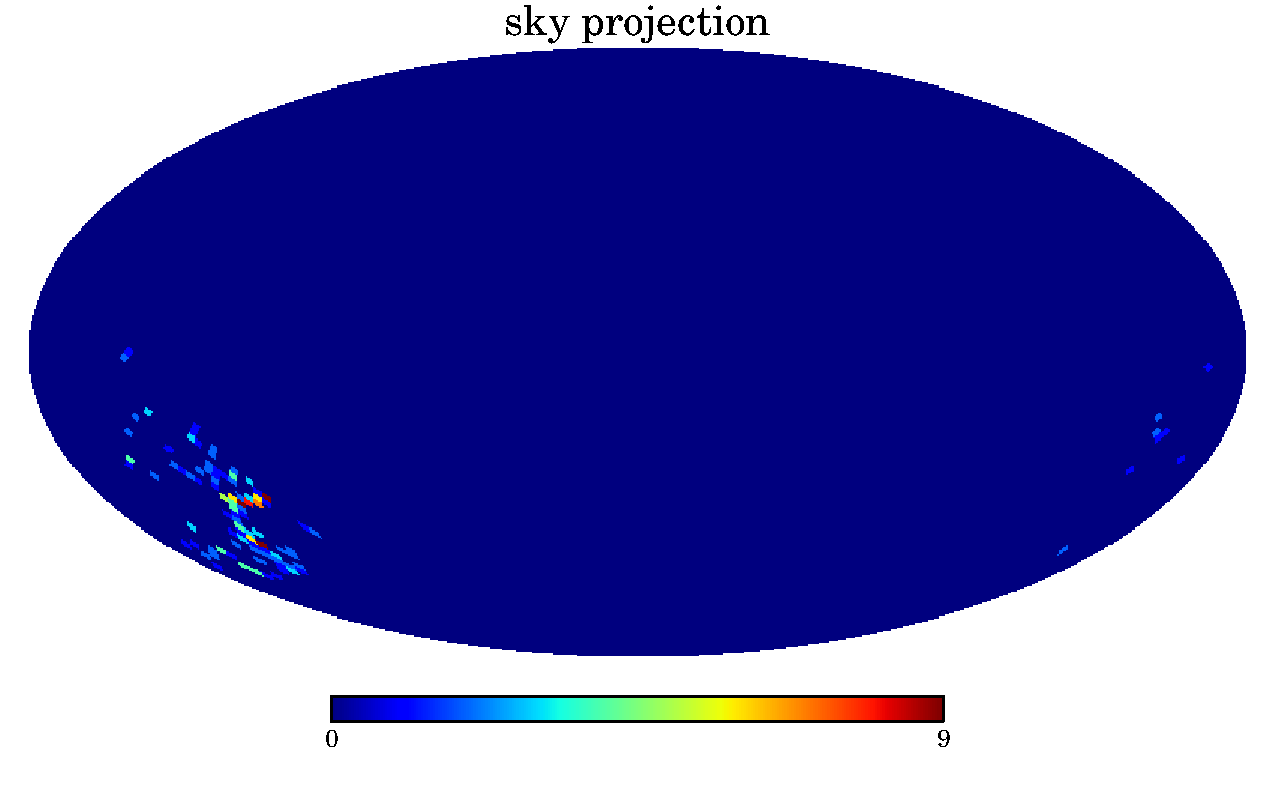
\includegraphics[width=12cm]{./Output/plots/HEALPix/sky_projection_HEALPix_Count_32.pdf}
 \caption{Plot of sky projection.}
 \label{fig:S-ProjCount}
\end{figure}

 .... 
\section*{ACKNOWLEDGMENTS}
 Arya Farahi wants to thank ...
 
\end{document}
